\section{Results}\label{sec:results}
The learning curves in Figure~\ref{fig:dshift_offline_normal} show the
$Q$-values evolution for the standard agents as a result of offline
training, while the ones in Figure~\ref{fig:dshift_offline_ensemble}
show the same metric for their respective ensemble version. Every
proposed offline agent learns to solve both classic control
environments, and the reward curves are presented in
Appendix~\ref{sec:appendix}.
% NOTE maybe this sentence is not even necessary
The reward signals for the \texttt{CartPole-v1} environment are
noisier compared to the ones for \texttt{Acrobot-v1}; this is in line
with the performance of the online behavioral DQN agent, which also
produced quite unstable learning curves on this problem.

\subsection{Offline bootstrapping error in the DQV family}
\begin{figure}[!tbp]
  \centering
  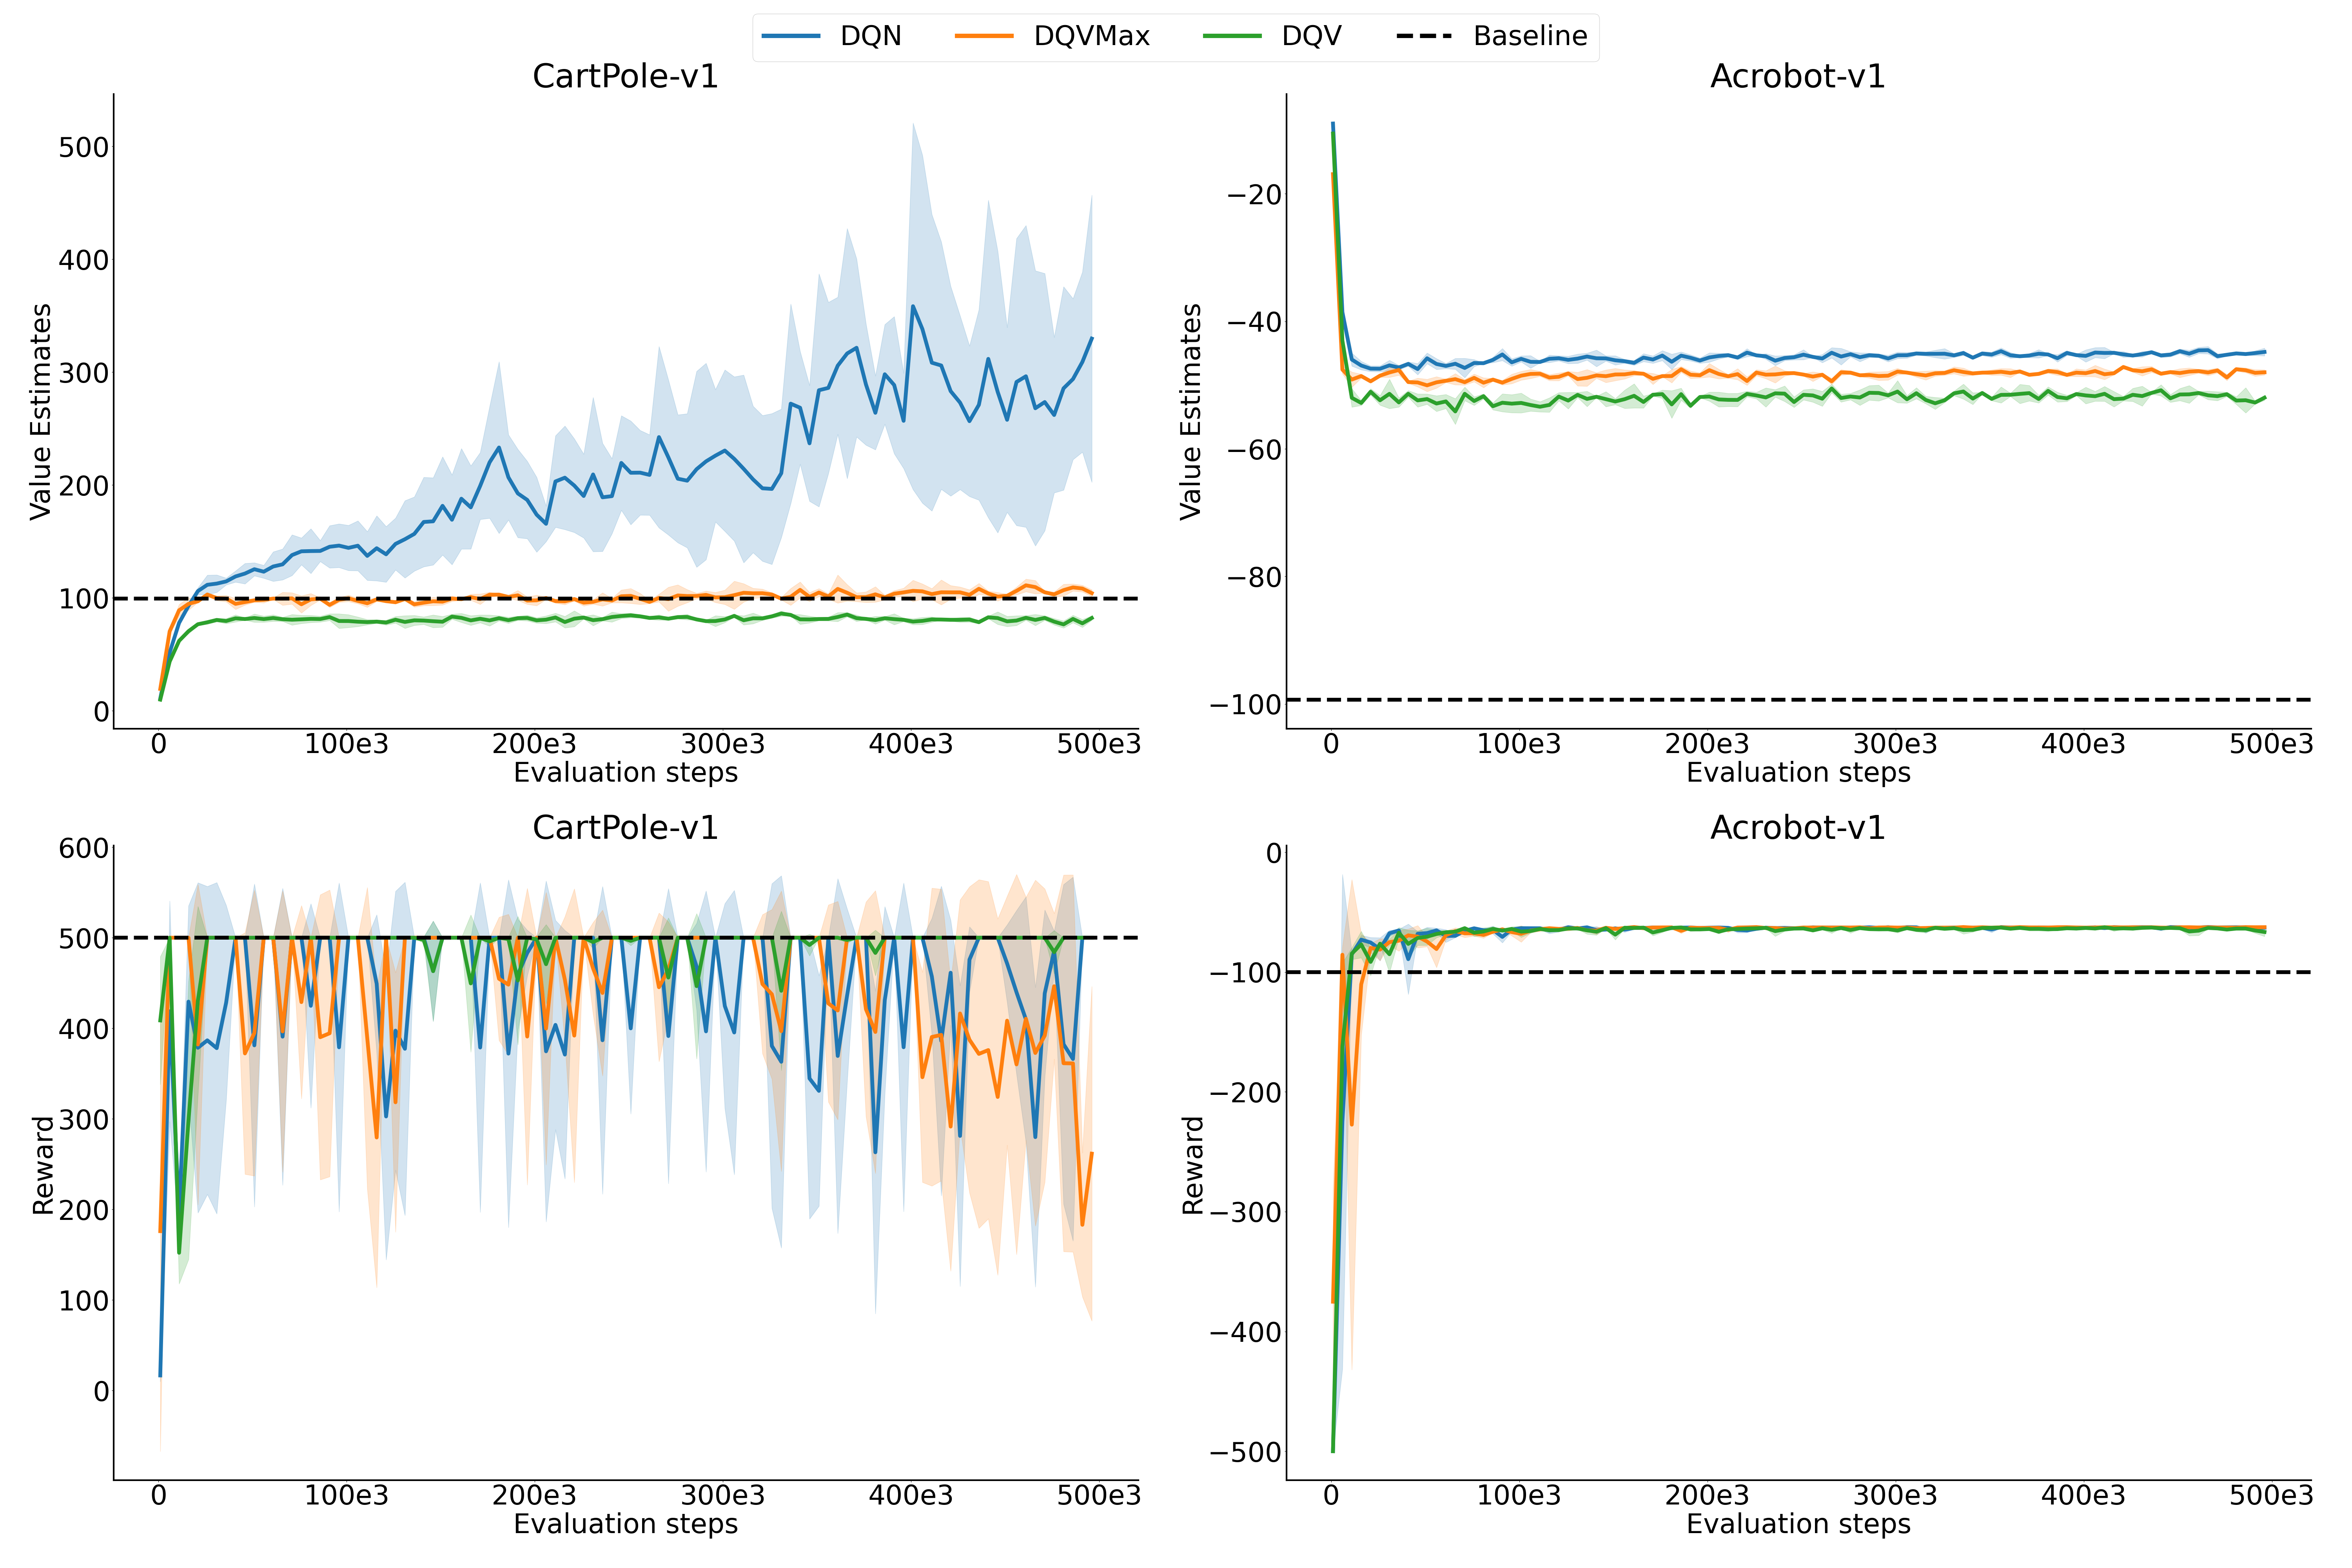
\includegraphics[width=.5\textwidth]{img/dshift_plots_normal.png}
  \caption{The $Q$-value estimates of offline DQN, DQV and DQV-Max at
    evaluation time. The shaded areas are $\pm 1$ standard deviation
    from the mean of 3 different
    simulations.}\label{fig:dshift_offline_normal}
\end{figure}
% Q estimates discussion for:
% DQN offline
% NOTE why no BE on acrobot for DQN offline? maybe the env is too easy
% TODO say something about acrobot too, where no BE seems to occur?
As seen in~\ref{fig:dshift_offline_normal}, the experiments confirmed
previous findings for Q-learning-based gents run offline on continuous
domain problems \citep{pmlr-v97-fujimoto19a,kumar2019stabilizing}: the
$Q$ function incurs in a heavy overestimation bias produced by
bootstrapping errors. This is most evident on the \texttt{CartPole-v1}
environment, where DQN's $Q$-value estimates quickly escalate above
the true value. Since the offline agent has no access to ground truth
values due to lack of exploration, it cannot adjust the $Q$ function
estimates during training and the whole estimation process diverges.

% DQV offline
% NOTE why dqv high BE or OB but still good performance on DQV?!
% motivate
% NOTE also, how is it possible that an on-policy algo is able to learn
% from off-policy data?
Among the studied algorithms, offline DQV is the most robust one to
the bootstrapping error. On the \texttt{CartPole-v1} environment it is
almost able to correctly estimate the true value of $s_0$ for each
episode, consistently assessing at approximately $-10$ points from the
true solution. However, on the \texttt{Acrobot-v1} problem, offline
DQV still suffers from a stable form of overestimation, despite coming
closest to the true value estimate of$ s_0$. DQV is likely capable of
resisting the bootstrapping error because it is an \textit{on-policy}
algorithm. Although theoretically it should not be able to learn in
the offline setting, its strong
performance compared to the other agents is probably due to efficient
usage of the large offline dataset, which enables it to learn on-policy
discovering effective behaviors in the data. Moreover, DQV forms its
TD-target using only the state-value function $V$, therefore it cannot
possibly base predictions on those very out-of-distribution actions
which are responsible for bootstrapping errors.

% DQV-Max offline
Offline DQV-Max is also more resilient to the bootstrapping error than
offline DQN.\ On the \texttt{CartPole-v1} environment, it estimates
the true value for $s_0$ nearly perfectly, showing no detrimental
effects due to misaligned bootstrap estimates. As it is the case for
offline DQV and DQN, it still overestimates the real $Q$-value for
$s_0$ on the \texttt{Acrobot-v1} problem, positioning in between the
estimates of DQN and DQV.\ The low $Q$-values on the
\texttt{CartPole-v1} environment are most likely in virtue of
DQV-Max's decoupling of \textit{selection} and \textit{evaluation}
\citep{van2016deep}. DQV-Max forms its temporal difference regression
targets (selection) from a model different than the one it uses to
compute value estimates (evaluation). This separation is especially
important for DQV-Max's TD-targets for the $V$ function of
Equation~\ref{dqvmax:v_td_target}, where evaluating
out-of-distribution actions could disrupt the function's
convergence to the true $V^*$. \citet{sabatelli2020deep} note that
this disentanglement makes DQV-Max less prone to the overestimation
bias in the online setting, and these experiments confirm the results
for the offline one.

\subsection{Offline bootstrapping error on the ensemble variants}
\begin{figure}[!tbp]
  \centering
  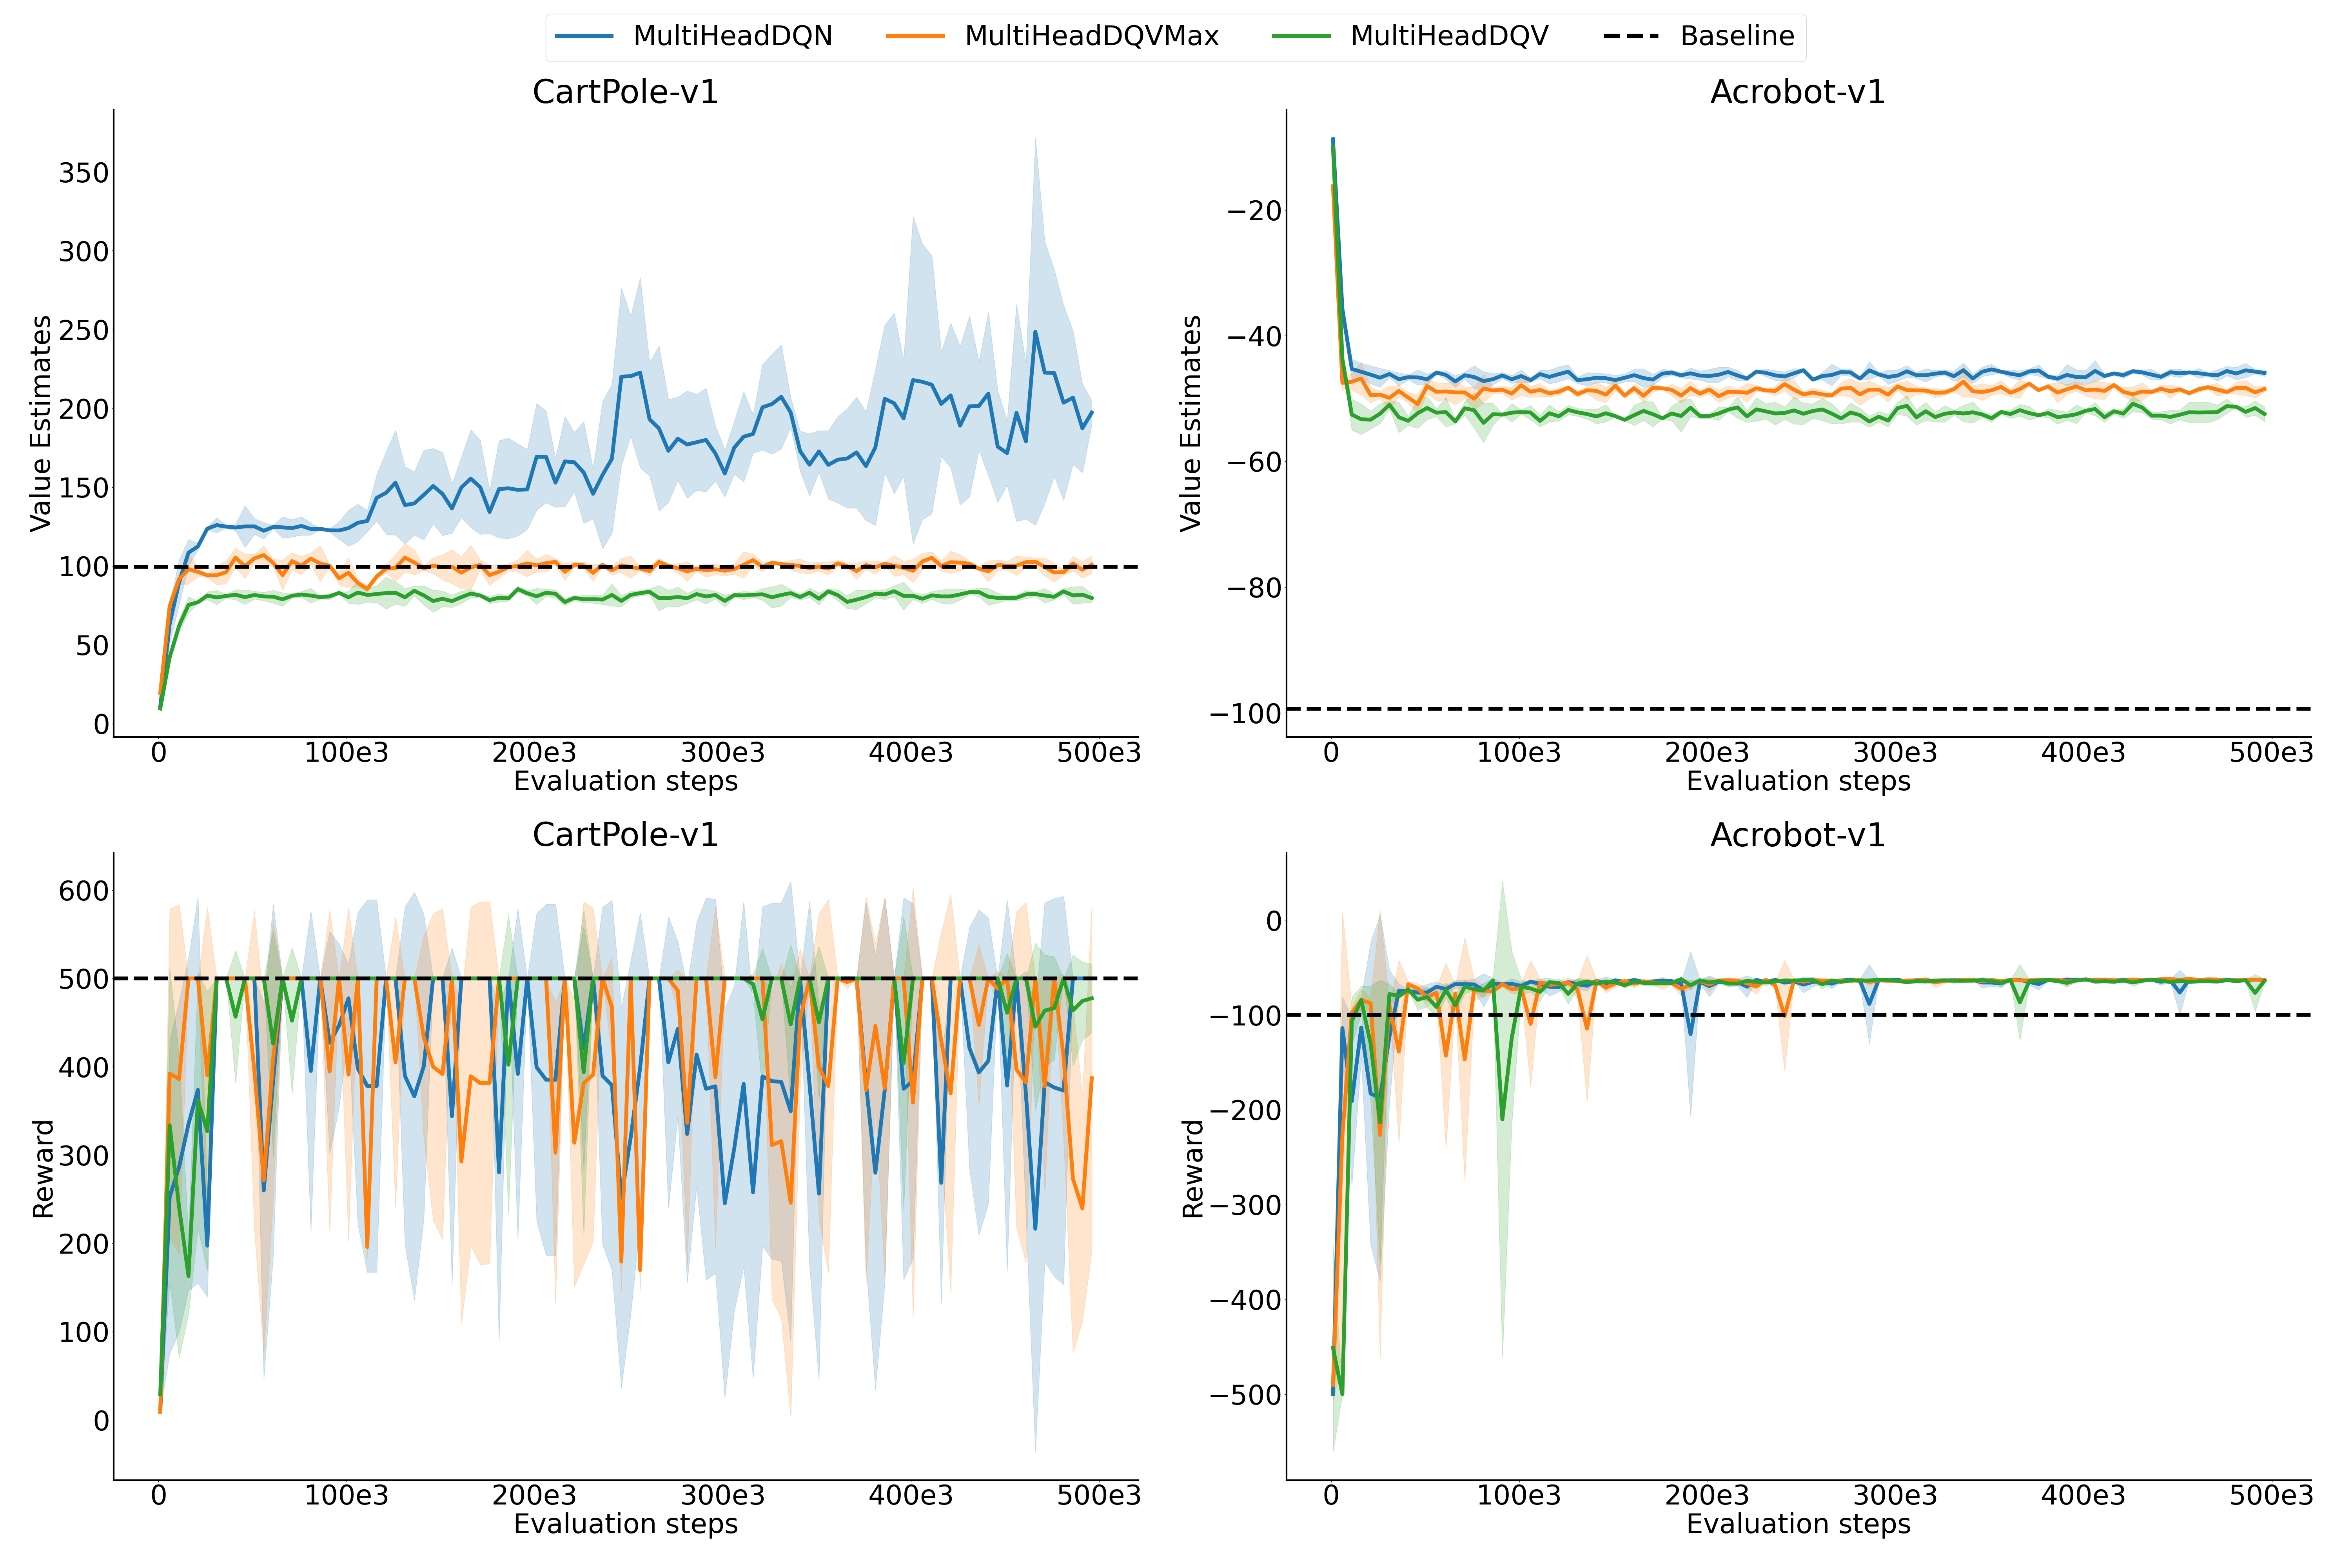
\includegraphics[width=.5\textwidth]{img/dshift_plots_ensembles.png}
  \caption{Evaluation time $Q$-value estimates of the ensemble version
    of offline DQN, DQV and DQV-Max. The shaded areas are $\pm 1$
    standard deviation from the mean of 3 different
    simulations.}\label{fig:dshift_offline_ensemble}
\end{figure}
% TODO I am not sure that the significance results are correct, there
% are too many significant differences! should I present the result in
% the table??
% TS: ensemble-dqn less optimistically biased, in line with baseline
% results from REM and with theoretical analysis of Averaged-DQN
Offline Ensemble-DQN suffers from a milder overestimation bias than
offline DQN.\ A significant reduction in $Q$-value estimates was
found on the ensemble version for both environments ($U=57775.0$ and
$U=57227.5$ respectively, $p<.01$). Moreover, on the
\texttt{CartPole-v1} environment, the $Q$ estimates of Ensemble-DQN
show approximately 4 times lower variance than those of DQN (8755.07
vs. 2330.90, respectively), in line with the aforementioned analysis
by \citet{anschel2017averaged}.

% stuff to say generally:
% - acrobot is more stable env for mean q values + for dqns and dqvs,
% variance too
% - generally: all algos seem to perform worse on ensemble version,
% and except for dqns, their estimates of the response metric have
% higher variability -> in fact also rewards are lower
% - differences are significant on the acrobot env for every algo ->
% why? dqvs q-values for variance likely, dqvmaxs seem the same
% though?!
 % - need to talk about the ablated versions: no significant differences
% at all, why is that?


% TS: ensemble-dqv no real change
Concerning offline Ensemble-DQV, no significant change to its standard
counterpart was observed as it can be seen from the nearly identical
$Q$-value curves of Figure~\ref{fig:dshift_offline_ensemble}. However,
the reward signals for this agent follow a pattern generally recorded
across all ensemble variants: average returns are more unstable across

% TODO paper plots:
% - standard algos offline, only Q-values
% - ensemble algos offline, only Q-values
% - DQVMax and ablations offline, only Q-values
% appendix:
% - rewards for standard agents
% - rewards for all ensemble agents (or should I exclude ablations?)
